\section{Komplexe Zahlen}
\subsection{Grundlagen}
\begin{center}
	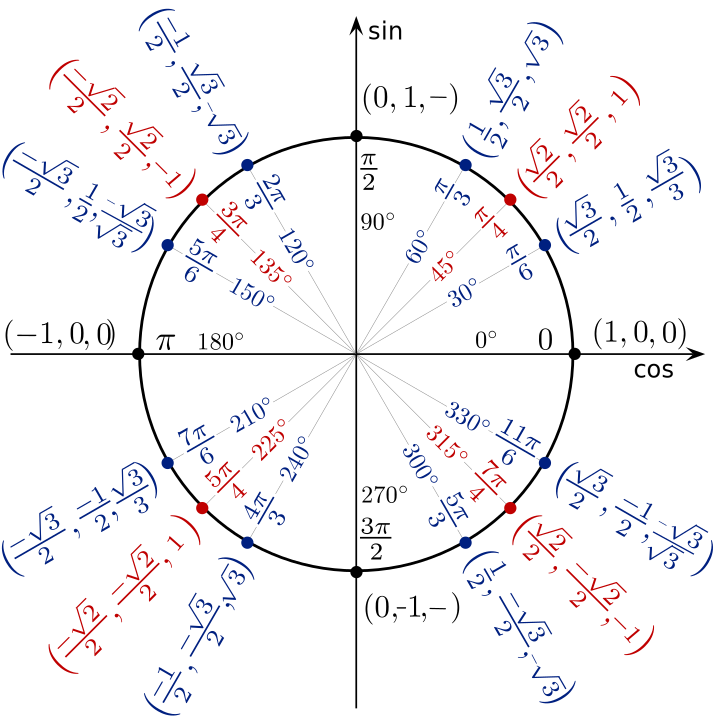
\includegraphics[width=0.6\columnwidth]{Images/einheitskreis}\\
	Punkte auf Kreis [$\cos(\alpha), \sin(\alpha), \tan(\alpha)$]
\end{center}

\begin{center}
	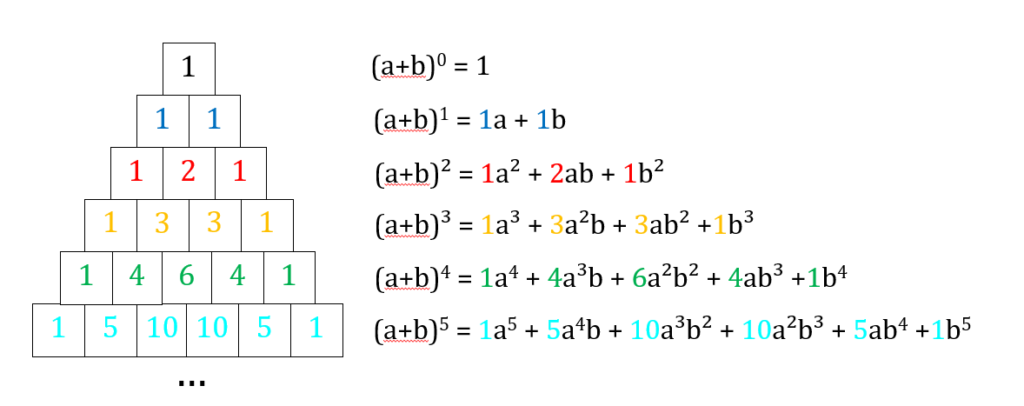
\includegraphics[width=\columnwidth]{Images/pascaldreieck}\\
\end{center}


\subsection{Operationen}
\noindent\textbf{Realteil}\\
$\Re(a) = a_1$\\

\noindent\textbf{Imaginärteil}\\
$\Im(a) = a_2$\\

\noindent\textbf{Komplex Konjugiert}\\
$\overline{a} = a^* = \overline{a_1 + ja_2} = a_1 - ja_2$\\

\noindent\textbf{Betrag}\\
$\left|a\right| = r = \sqrt{\Re(a)^2 + \Im(a)^2} = \sqrt{a_1^2 + a_2^2} $\\

\noindent\textbf{Argument}\\
$\arg(a) = \zeta = \left\{\begin{array}{ll}
	a_2 \geq 0 ,& \arccos\left(\frac{a_1}{r}\right) \text{ oder } \arctan\left(\frac{a_1}{a_2}\right)\\
	a_2 < 0 ,& -\arccos\left(\frac{a_1}{r}\right) \text{ oder } \arctan\left(\frac{a_1}{a_2}\right) + \pi\\
\end{array}\right.$\\


\subsubsection{Kartesisch}
In diesem Koordinatensystem lassen sich \textit{Addition} und \textit{Subtraktion} besonders einfach lösen!

\noindent\textbf{Addition}\\
$(a_1 + ja_2) + (b_1 + jb_2) = a_1 + ja_2 + b_1 + jb_2 = (a_1 + b_1) + j(a_2 + b_2)$\\

\noindent\textbf{Subtraktion}\\
$(a_1 + ja_2) - (b_1 + jb_2) = a_1 + ja_2 - b_1 - jb_2 = (a_1 - b_1) + j(a_2 - b_2)$\\

\noindent\textbf{Multiplikation} (Binom.)\\
$(a_1 + ja_2) \cdot (b_1 + jb_2) = (a_1b_1 - a_2b_2) + j(a_1b_2 + a_2b_1)$\\

\noindent\textbf{Division}\\
$\frac{a_1 + ja_2}{b_1 + jb_2} = \frac{(a_1 + ja_2)}{(b_1 + jb_2)} \cdot \underbrace{\frac{(b_1 - jb_2)}{(b_1 - jb_2)}}_{\overline{b} = \text{komplex konj.}} = \frac{1}{b_1^2 + b_2^2}(a_1+ja_2)(b_1 - jb_2)$\\

\subsubsection{Polar}
In diesem Koordinatensystem lassen sich \textit{Multiplikation} und \textit{Division} besonders einfach lösen!

\noindent\textbf{Multiplikation $a \cdot b = c$}\\
$\Re(c) = |a_1| \cdot |b_1| \qquad \Im(z) = \arg(a_2 \cdot b_2) = \arg(a_2) + \arg(b_2)$\\

\noindent\textbf{Division  $\frac{a}{b} = c$}\\
$\Re(c) = \frac{a_1}{b_1} \qquad \Im(z) = \arg(\frac{a_2}{b_2}) = \arg(a_2) - \arg(b_2)$\\

\noindent\textbf{Potenz ($n \in \mathbb{N}$)}, für $n \in \mathbb{C}$ siehe \ref{potfunc}\\
$a^n = r^n \cdot [\cos(\zeta) + j\sin(\zeta)]^n = r^n \cdot [\cos(n\zeta) + j\sin(n\zeta)]$\\

\noindent\textbf{n-te Wurzel}\\
$z_{k+1} = \sqrt[n]{r} \cdot \cjs\left(\frac{2\pi}{n} + k \cdot \frac{2\pi}{n}\right) \qquad k \in (0, 1, \cdots, n-1)$

~\\
\noindent\textbf{Hinweis:} Diese Punkte $z_{k+1}$ liegen im Abstand von $\sqrt[n]{r}$ zum Ursprung als regelmässiges n-Eck angeordnet. Alle $\Im(z_{k+1}) \neq 0$ \underline{müssen} konjugiert komplex sein (Vorzeichenwechsel von $\Im$ Komponente)! Reelle Lösungen treten nur einzeln auf. 

\subsection{Polarform Umwandlung}
Beispiel Format:
\[
z = z_1+ jz_2 \xRightarrow[]{\text{Polar (Trigo)}} r \cdot \left[\cos(\zeta) + j\sin(\zeta)\right] \xRightarrow[]{\text{Euler}} r \cdot e^{\zeta j}
\]
\begin{center}
	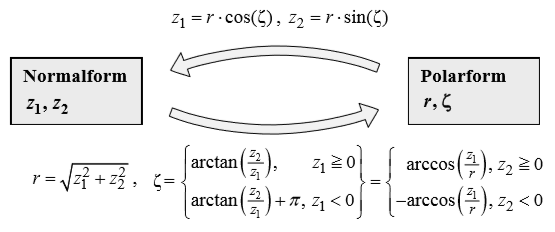
\includegraphics[width=0.6\columnwidth]{Images/umwandlung}
\end{center}

\subsection{Ebene Geometrie}
\subsubsection{Vektoren}
\begin{minipage}{\textwidth}		
	\begin{minipage}{0.2\textwidth}
		\textbf{Addition/Subtraktion}\\
		Ortsvektoren und Strecken können gleich wie Vektoralgebra berechnet werden.
	\end{minipage}%%% to prevent a space
	\begin{minipage}{0.3\textwidth}
		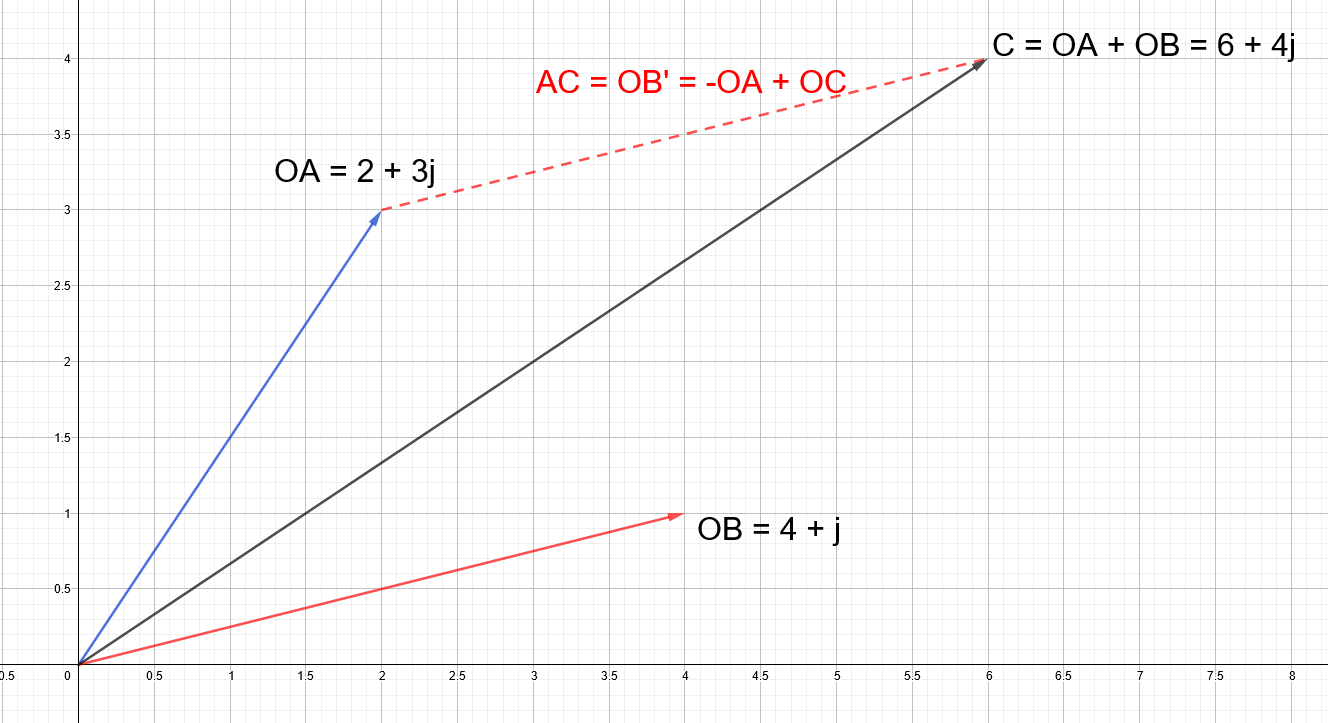
\includegraphics[width=\columnwidth]{Images/vec_addition}
	\end{minipage}
\end{minipage}
~\\
\begin{minipage}{\textwidth}		
	\begin{minipage}{0.2\textwidth}
		\textbf{Multiplikation}\\
		Erreicht eine Drehung der Strecke $AB$ um Winkel $\cjs(\zeta)$
	\end{minipage}%%% to prevent a space
	\begin{minipage}{0.3\textwidth}
		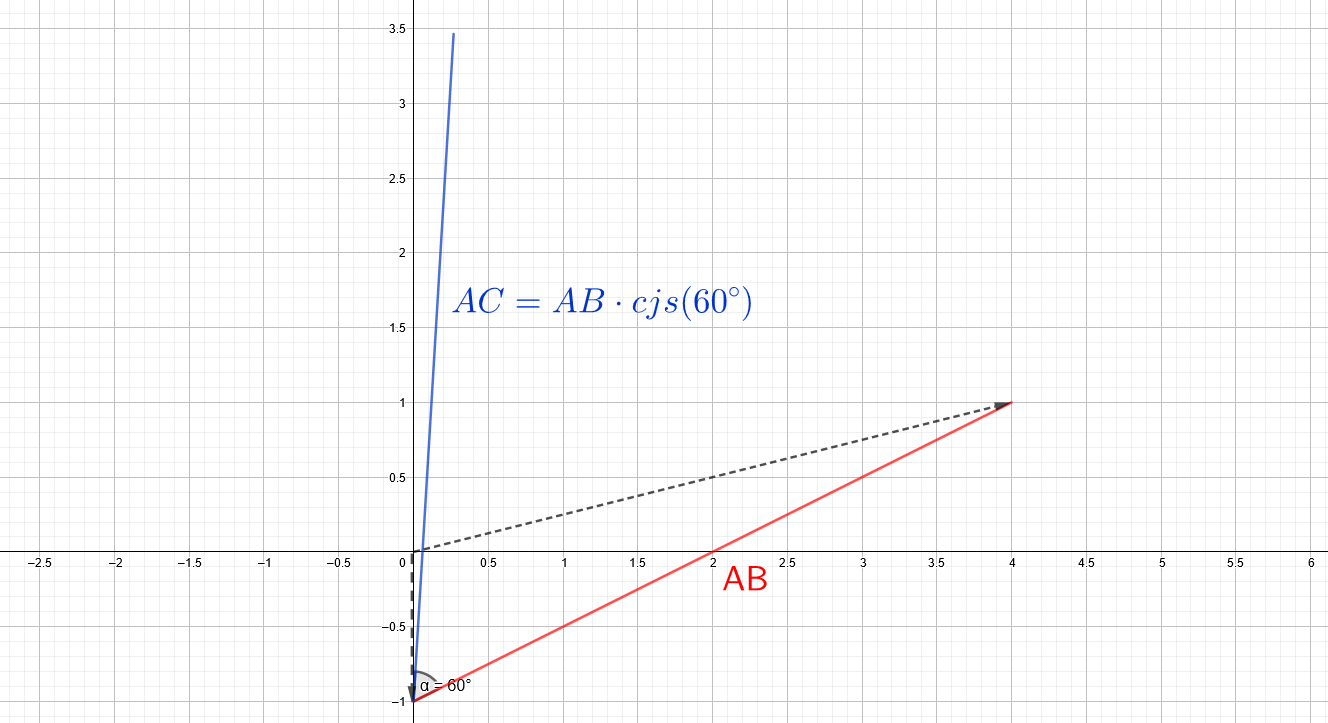
\includegraphics[width=\columnwidth]{Images/vec_multiplikation}
	\end{minipage}
\end{minipage}
